% !TEX root = ../thesis-example.tex
%
\chapter{Evaluation}
\label{sec:evaluation}

\Blindtext[2][1]

\section{Experimental setup}

\Blindtext[2][1]



\section{System evaluation}

In this section we present the performance evaluation of the proposed system.

\subsection{Performance and cost evaluation}
\label{sec:perf}



\begin{figure}[h]
  \centering
  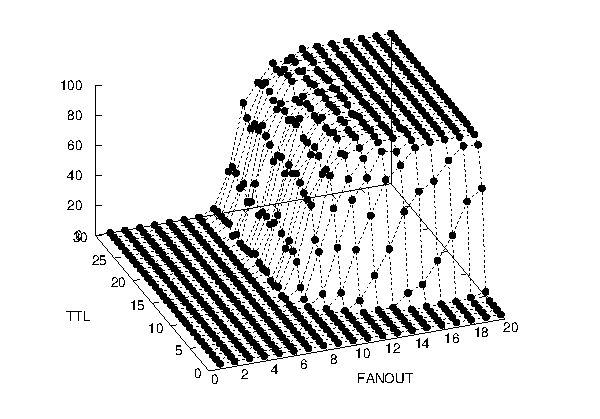
\includegraphics{figs/complete.pdf}
  \caption{This figure shows the percentage of complete disseminations.}
  \label{fig:complete}
\end{figure}

\Blindtext[2][1]

\begin{figure}[h]
  \centering
  \begin{subfigure}[b]{0.45\linewidth}
    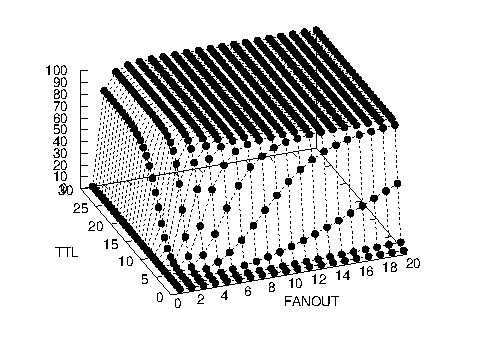
\includegraphics{figs/hitratio.pdf}
  \end{subfigure}
  \hspace{1cm}
  \begin{subfigure}[b]{0.45\linewidth}
    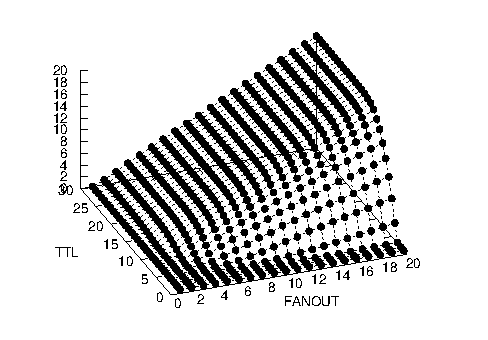
\includegraphics{figs/redundant.pdf}
  \end{subfigure}
  \caption{These are the remaining two figures.}
  \label{fig:others}
\end{figure}

Note the detail in Figures~\ref{fig:complete} and~\ref{fig:others}.




Table~\ref{table:my_test_table} is a test table, listing all numbers from 1 to 9.

\begin{table}
  \centering
  \begin{tabular}{||c||c||c||}
    \hline
    First column & Second column & Third column \\ [0.5ex] 
    \hline\hline
    1 & 2 & 3 \\ 
    \hline
    4 & 5 & 6 \\ 
    \hline
    7 & 8 & 9 \\ [1ex]
    \hline
  \end{tabular}
  \caption{Test table}
  \label{table:my_test_table}
\end{table}


\Blindtext[1][1]





\subsection{Qualitative evaluation}
\label{sec:qual_eval}

\Blindtext[2][1]





\subsection{Effect of other parameters}
\label{sec:concepts:sec2}

\Blindtext[2][1]
